\documentclass{article}
\usepackage[utf8]{inputenc}
\usepackage[margin=1in]{geometry}
\usepackage{listings}
\usepackage{xcolor}
\usepackage{booktabs}
\usepackage{graphicx}


\definecolor{codegreen}{rgb}{0,0.6,0}
\definecolor{codegray}{rgb}{0.5,0.5,0.5}
\definecolor{codepurple}{rgb}{0.58,0,0.82}
\definecolor{backcolour}{rgb}{0.95,0.95,0.92}

\lstdefinestyle{mystyle}
{
	backgroundcolor=\color{backcolour},   
	commentstyle=\color{codegreen},
	keywordstyle=\color{magenta},
	numberstyle=\tiny\color{codegray},
	stringstyle=\color{codepurple},
	basicstyle=\ttfamily\footnotesize,
	breakatwhitespace=false,         
	breaklines=true,                 
	captionpos=b,                    
	keepspaces=true,                 
	numbers=left,                    
	numbersep=5pt,                  
	showspaces=false,                
	showstringspaces=false,
	showtabs=false,                  
	tabsize=2
}

\lstset{style=mystyle}
\begin{document}
\begin{titlepage} % Suppresses displaying the page number on the title page and the subsequent page counts as page 1
	
	\raggedleft\rule{1pt}{\textheight} % Vertical line
	\hspace{0.05\textwidth} % Whitespace between the vertical line and title page text
	\parbox[b]{0.75\textwidth}
	{ % Paragraph box for holding the title page text, adjust the width to move the title page left or right on the page
		
		{\Huge\bfseries MIT World Peace University \\[0.5\baselineskip] \ Advanced Data Structures}\\[2\baselineskip] % Title
		{\large\textit{Assignment 5}}\\[4\baselineskip] % Subtitle or further description
		{\Large\textsc{Naman Soni Roll No. 10}} % Author name, lower case for consistent small caps
		
		\vspace{0.5\textheight} % Whitespace between the title block and the publisher
	}
	
\end{titlepage}
\tableofcontents
\pagebreak
\section{\textbf{Problem Statement}}
Consider a friend’s network on Facebook social web site. Model it as a graph to represent each
node as a user and a link to represent the friend relationship between them using adjacency list
representation and perform DFS and BFS traversals.
\section{\textbf{Objective}}
\begin{enumerate}
    \item To study data structure Graph and its representation using adjacency list
    \item To study and implement recursive Depth First Traversal and use of stack data structure for recursive Depth First Traversal
    \item To study and implement Breadth First Traversal
    \item To study how graph can be used to model real world problems
\end{enumerate}
\section{\textbf{Theory}}
\subsection{\textit{Graph and its types}}
Graphs are used to represent complex relationships between data elements. Graphs can be directed or undirected, and can have weighted edges or unweighted edges.\\
Some common operations on graphs include traversal (visiting all the vertices in the graph), shortest path finding (finding the shortest path between two vertices), and minimum spanning tree finding (finding a subset of edges that form a tree that connects all vertices in the graph with minimum total weight).\\
Graph algorithms are used in many areas of computer science, such as network optimization, social network analysis, computational biology, and artificial intelligence. Some common graph algorithms include Breadth-First Search, Depth-First Search, Dijkstra's Algorithm, and Kruskal's Algorithm.\\
There are 5 types of graphs:
\begin{itemize}
    \item \textbf{Directed Acyclic Graph (DAG):} A DAG is a directed graph that contains no directed cycles. That is, it is impossible to start at any vertex and follow a sequence of edges that eventually loops back to the starting vertex. DAGs are used to model dependencies between tasks or events, and are commonly used in scheduling and resource allocation problems.
        \begin{center}
            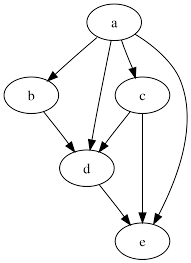
\includegraphics[width=0.3\textwidth]{DAG.png}
        \end{center}
    \pagebreak
    \item \textbf{Weighted Graph:} A weighted graph is a graph in which each edge is assigned a numerical weight or cost. Weighted graphs are used to represent many types of real-world networks, such as transportation networks, social networks, and communication networks. They are also used in optimization problems, such as the shortest path problem and the minimum spanning tree problem.
        \begin{center}
            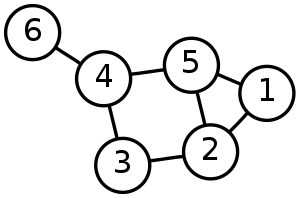
\includegraphics[width=0.3\textwidth]{WG.png}
        \end{center}
    \item \textbf{Bipartite Graph:} A bipartite graph is a graph whose vertices can be divided into two disjoint sets, such that every edge connects a vertex from one set to a vertex from the other set. Bipartite graphs are used to represent many types of relationships, such as buyers and sellers in a market, students and classes in a university, and books and authors in a library.
        \begin{center}
            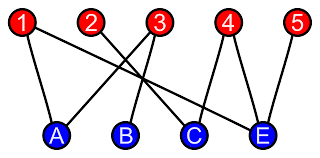
\includegraphics[width=0.4\textwidth]{BG.png}
        \end{center}
    \item \textbf{Complete Graph:} A complete graph is a graph in which every pair of distinct vertices is connected by an edge. Complete graphs are used to model many types of networks, such as social networks, communication networks, and transportation networks. They are also used in optimization problems, such as the traveling salesman problem.
        \begin{center}
            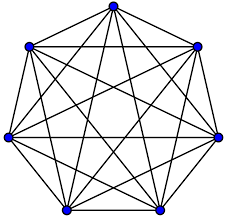
\includegraphics[width=0.3\textwidth]{CG.png}
        \end{center}
    \item \textbf{Spanning Tree:} A spanning tree of a connected graph is a tree that includes all of the graph's vertices and a subset of its edges, such that the tree is connected and acyclic. Spanning trees are used to represent many types of relationships, such as hierarchies in organizations and networks of roads or pipelines.
        \begin{center}
            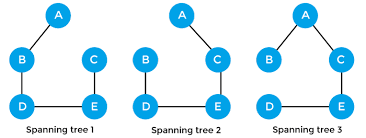
\includegraphics[width=0.4\textwidth]{ST.png}
        \end{center}
\end{itemize}
\subsection{\textit{Representation of graph using adjacency list with one example and diagram.}}
One common way to represent a graph in computer science is using an adjacency list. In this representation, each vertex in the graph is associated with a list of its neighboring vertices. Here's an example of a graph and its corresponding adjacency list representation:\\
\begin{figure}[h]
    \centering
    \includegraphics[width=0.5\textwidth]{undirectedgraph.png}
    \caption{Undirected Graph}
\end{figure}

An array of linked lists is used. The size of the array is equal to the number of vertices. Let the array be an array[ ]. An entry array[i] represents the linked list of vertices adjacent to the ith vertex. This representation can also be used to represent a weighted graph. The weights of edges can be represented as lists of pairs. Following is the adjacency list representation of the above graph.
\begin{figure}[h]
    \centering
    \includegraphics[width=0.5\textwidth]{listadjacency.png}
    \caption{Adjacency List}
\end{figure}
\subsection{\textit{Graph Traversals DFT and BFT with example and diagrams}}
Graph traversal refers to the process of visiting all vertices in a graph. There are two common methods for traversing a graph: Depth-First Traversal (DFT) and Breadth-First Traversal (BFT).\\

\textbf{Depth-First Traversal:} In DFT, we start at a vertex and visit as far as possible along each branch before backtracking. This process continues until all vertices have been visited. Here's an example of DFT on a graph:
\begin{lstlisting}
     2
    / \
   0   3
   | \  \
   1  4  5

\end{lstlisting}
\pagebreak
Starting at vertex 2, we follow the first branch until we reach vertex 0. From there, we continue exploring along the first branch until we reach vertex 1. Since vertex 1 has no more unexplored neighbors, we backtrack to vertex 0 and continue along the second branch, visiting vertex 4. Finally, we backtrack to vertex 2 and continue along the second branch, visiting vertex 3 and then vertex 5.\\

The order in which we visited the vertices in this example is: `2, 0, 1, 4, 3, 5'.\\

Here's a diagram illustrating the DFT process:
\begin{lstlisting}
    Step 1:
        2
       / \
      0   3
      | \  \
      1  4  5

Visited: 2

Step 2:
        2
       / \
      0   3
      | \  \
      1  4  5

Visited: 2, 0

Step 3:
        2
       / \
      0   3
      | \  \
      1  4  5

Visited: 2, 0, 1

Step 4:
        2
       / \
      0   3
      | \  \
      1  4  5
Visited: 2, 0, 1, 4
Step 5:
        2
       / \
      0   3
      | \  \
      1  4  5

Visited: 2, 0, 1, 4, 3

Step 6:
        2
       / \
      0   3
      | \  \
      1  4  5

Visited: 2, 0, 1, 4, 3, 5

\end{lstlisting}
\pagebreak
\textbf{Breadth-First Traversal:} In BFT, we start at a vertex and visit all of its neighbors before moving on to any of their neighbors. This process continues until all vertices have been visited. Here's an example of BFT on a graph:\\

Starting at vertex 2, we visit all its neighbors first: vertices 0 and 3. Then, we visit all the neighbors of vertices 0 and 3: vertices 1, 4, and 5. The order in which we visited the vertices in this example is: `2, 0, 3, 1, 4, 5'.\\
Here's a diagram illustrating the BFT process:
\begin{lstlisting}
    Step 1:
        2
       / \
      0   3
      |    \
      1     5
           /
          4

Visited: 2

Step 2:
        2
       / \
      0   3
      |    \
      1     5
           /
          4

Visited: 2, 0, 3

Step 3:
        2
       / \
      0   3
      |    \
      1     5
           /
          4

Visited: 2, 0, 3, 1, 4

Step 4:
        2
       / \
      0   3
      |    \
      1     5
           /
          4

Visited: 2, 0, 3, 1, 4, 5
\end{lstlisting}
\section{\textbf{Implementation}}
\subsection{\textit{Platform}}
\begin{itemize}
	\item 64-bit Mac OS
	\item Open Source C++ Programming tool like Visual Studio Code
\end{itemize}
\subsection{\textit{Test Conditions}}
\begin{enumerate}
    \item Input at least 5 nodes.
    \item Display DFT (recursive and non recursive)and BFT
\end{enumerate}
\section{\textbf{Conclusion}}
Thus, we have represented graph using adjacency list and performed DFT and BFT on it. We have also discussed the time complexity of the algorithms.
\section{\textbf{FAQ's}}
\subsection{\textit{Explain two applications of graph.}}
\textbf{Ans.} Graphs are a powerful data structure that can be used to model and solve a wide variety of problems. Here are two common applications of graphs:
\begin{enumerate}
    \item \textbf{Social Networks:} Graphs are widely used to model social networks such as Facebook, LinkedIn, and Twitter. In a social network, each user is represented as a node in the graph, and the relationships between users (such as friendship, following, or connection) are represented as edges. This graph can be used to analyze the structure of the social network, identify influential users or communities, and suggest new connections or friends for a user.
    \item \textbf{Routing and Navigation:} Graphs can also be used to model road networks, transportation systems, and other types of networks where routes need to be optimized. In this case, each intersection or location is represented as a node in the graph, and the roads or connections between them are represented as edges. Using graph algorithms such as Dijkstra's algorithm or the A* algorithm, it is possible to find the shortest path or fastest route between two locations on the network. This can be used for navigation systems, logistics optimization, and other applications where efficient routing is important.
\end{enumerate}
\subsection{\textit{Explain advantages of adjacency list over adjacency matrix.}}
\textbf{Ans.} Adjacency matrix and adjacency list are two common ways to represent graphs in computer science. Here are some advantages of using an adjacency list over an adjacency matrix:
\begin{enumerate}
    \item Space efficiency: Adjacency lists are more space-efficient than adjacency matrices, especially for sparse graphs. In an adjacency matrix, we have to allocate space for every possible edge, even if the edge does not exist in the graph. For a sparse graph, this can lead to a lot of wasted space. In contrast, an adjacency list only stores the edges that actually exist in the graph, making it more space-efficient.
    \item Efficient iteration over neighbors: In an adjacency list, it is easy to iterate over the neighbors of a given vertex. We just need to iterate over the list of edges connected to that vertex. In contrast, in an adjacency matrix, we have to iterate over an entire row or column to find the neighbors of a vertex, which can be slower for large graphs.
    \item Easy addition and removal of edges: In an adjacency list, it is easy to add or remove edges from the graph. We just need to add or remove an edge from the list of edges for each vertex. In contrast, in an adjacency matrix, we have to update the entire row and column for each vertex whenever we add or remove an edge, which can be slower for large graphs.
    \item Memory allocation: Adjacency list requires memory allocation only for edges that exist, thus it is more flexible for dynamic allocation of memory.
\end{enumerate}
\pagebreak
\subsection{\textit{Why transversal in graph is different than traversal in tree}}
\textbf{Ans.} Traversal in a graph is different from traversal in a tree for several reasons:
\begin{enumerate}
    \item Multiple paths: In a tree, there is only one unique path from the root to any leaf node. However, in a graph, there can be multiple paths between two vertices. This means that a traversal algorithm for a graph must be able to handle the possibility of visiting a vertex multiple times along different paths.
    \item Loops and cycles: Graphs can contain loops or cycles, which means that a traversal algorithm may encounter the same vertex or edge more than once during the traversal. In contrast, trees do not contain loops, so a traversal algorithm for a tree does not need to check for cycles.
    \item Connected components: A graph can be disconnected, meaning that there are two or more separate subgraphs that are not connected by any edges. In this case, a traversal algorithm must be able to visit each connected component separately. In contrast, a tree is always a single connected component.
    \item Undefined root: A tree always has a well-defined root node, but a graph does not. This means that a traversal algorithm for a graph must be able to start from any vertex in the graph.
\end{enumerate}
\end{document}